% ============================================================
%  SECTION 8: Nominal and real exchange rates, PPP  (Member 3)
%  Member 3's text. Changes at merge:
%   - Maharaja Mac: undervaluation corrected to about 53 per cent (was "over 40%")
%   - GNI box updated to World Bank 2025 data (Macrotrends source removed)
%   - new figure drawing the worked example
% ============================================================
\section{Nominal and real exchange rates, and purchasing power parity}\label{sec:real}

So far, we have talked about the exchange rate as a single number: how many rupees it takes to buy one US dollar. This is called the \keyterm{nominal exchange rate}{The number of rupees needed to buy one unit of foreign currency, as quoted in the market.}, and it is what you see on a currency exchange board or a news ticker. However, this number alone does not tell the full story of a currency's strength.

Consider this: suppose the nominal exchange rate stays exactly the same, say ₹83 per US dollar, for an entire year. At first glance, nothing has changed. But if prices in India rise by 10 per cent over that year while prices in the US stay flat, Indian goods have become 10 per cent more expensive for American buyers, even though the exchange rate did not move. India has effectively become less competitive as an exporter, not because of any change in the exchange rate, but because of inflation at home. This is what the \keyterm{real exchange rate}{The nominal exchange rate adjusted for differences in price levels between two countries.} captures. It adjusts the nominal rate for differences in price levels between two countries. If Indian prices are rising faster than American prices, the real exchange rate is appreciating even when the nominal rate is unchanged, making Indian exports relatively more expensive.

\begin{workedexample}{How inflation changes the real exchange rate}
Suppose India and the US start the year with an exchange rate of ₹80 per US dollar. India experiences 8 per cent inflation while the US experiences 2 per cent inflation, and the nominal rate stays unchanged.

At the start of the year, a product priced at ₹800 in India costs \$10 in the US. By the end of the year, the same product costs ₹864 in India (up 8 per cent) but only \$10.20 in the US (up 2 per cent). At ₹80 per dollar, ₹864 converts to \$10.80, which is now more expensive than the \$10.20 US price (Figure~\ref{fig:realrate}). Indian exports have become less competitive even though the nominal exchange rate did not change at all. This is what it means for the real exchange rate to appreciate.
\end{workedexample}

\begin{figure}[!htb]
  \centering
  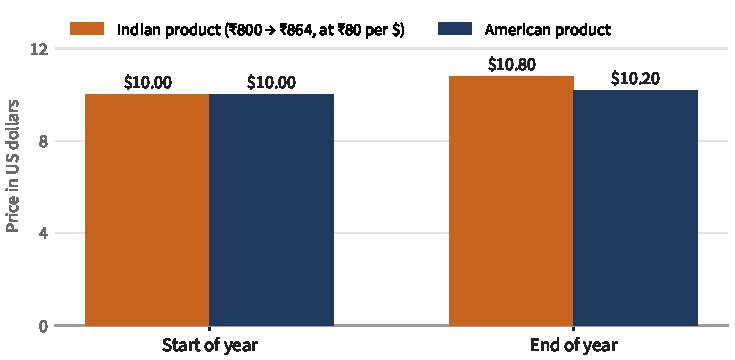
\includegraphics[width=\linewidth]{figures/real_rate.pdf}
  \caption{The same product, priced in dollars, before and after a year of inflation.}
  \label{fig:realrate}
  {\raggedright\small\sffamily The exchange rate stays at ₹80 per US dollar all year. Because prices rise faster in India, the Indian product overtakes its American rival in dollar terms.\par}
  \figsource{Drawn by the authors from the worked example. All values are hypothetical.}
\end{figure}

This idea connects directly to a concept called \keyterm{purchasing power parity (PPP)}{The idea that the same basket of goods should cost the same in every country once prices are converted into one currency.}. PPP is based on a simple idea: a basket of goods should cost the same in every country, once prices are converted into the same currency. If a basket of groceries costs ₹500 in India and \$6 in the US, then the PPP exchange rate would be roughly ₹83 per US dollar. If the actual exchange rate is very different from this, it suggests one currency is overvalued or undervalued.

However, PPP does not hold exactly in the real world. First, transport costs and import taxes mean that identical goods are not equally priced across borders. Second, many goods and services simply cannot be traded across countries at all. A haircut, a local bus ride, or a meal at a street stall in India costs far less than the equivalent in the US, not because of currency misalignment, but because these services are priced according to local wages and cannot be exported to equalise prices.

Despite its limitations, PPP is extremely useful for comparing living standards across countries. If you use the nominal exchange rate to compare incomes, a country with low prices appears poorer than it actually is. PPP adjustments correct for this by accounting for what money can actually buy in each country, giving a fairer picture of real living standards.

\begin{didyouknow}{The Maharaja Mac index}
Every year, \textit{The Economist} magazine publishes the Big Mac index, which compares the price of a McDonald's burger across countries to estimate whether currencies are overvalued or undervalued. Since beef is not widely eaten in India, McDonald's India sells a Maharaja Mac instead, and \textit{The Economist} uses its chicken version as India's entry in the index.

In January 2023, a Maharaja Mac cost ₹207 in India and a Big Mac cost \$5.36 in the US. This implies a PPP exchange rate of about ₹38.6 per US dollar, while the actual rate was around ₹81.7. This suggests the rupee was undervalued by about 53 per cent against the dollar, meaning money goes much further in India than the nominal exchange rate would suggest (The Economist, 2026).
\end{didyouknow}

\begin{didyouknow}{PPP and India's income}
India's nominal gross national income (GNI) per person, converted at market exchange rates, was about \$2,760 in 2025. Adjusted for PPP, it was about \$11,600, roughly 4.2 times higher (World Bank, 2026c). This gap exists because everyday goods and services in India are far cheaper than in high-income countries, so the same amount of money buys much more. International organisations like the World Bank and IMF prefer PPP figures when comparing living standards across countries for exactly this reason.
\end{didyouknow}
